\documentclass{article}

\usepackage[utf8]{inputenc}
\usepackage[L7x]{fontenc}
\usepackage[lithuanian]{babel}
\usepackage{lmodern}

\usepackage[usenames,dvipsnames]{xcolor}
\usepackage{tcolorbox}

\usepackage{amsmath}
\usepackage{media9}
\usepackage{graphicx}
\usepackage{animate}
%\usepackage{main}
%\usepackage{xstring}
\usepackage[top=2cm, bottom=2cm, left=2cm, right=2cm, footskip=1cm, a4paper]{geometry}
\usepackage{multirow}
\usepackage{verbatim}
\usepackage[tikz]{ocgx2}
\usepackage{pgfplots}
\usepackage{ifthen}
\usepackage{calc} 
\usepackage{indentfirst}
\usepackage{hyperref}
\usepackage{tikz}
\usetikzlibrary{positioning}% we need to add block on the right of next block
\usepackage{comment}

%This is a command that puts two minipage separated by \hspace{\fill}: two buttons in first minipage and gif in second minipage

\newcommand{\control}[2]{
\begin{minipage}[m]{0.05\linewidth}
\begin{tabular}{c}
\mediabutton[
mediacommand=#1:playPause,%
overface=\color{blue}{\fbox{\strut \includegraphics[width=\textwidth]{resumebut.png}}},
downface=\color{red}{\fbox{\strut \includegraphics[width=\textwidth]{resumebut.png}}}
]{\fbox{\strut \includegraphics[width=\textwidth]{playbut.png}}}\\
\mediabutton[
mediacommand=#1:setSource [(#1)],%
overface=\color{blue}{\fbox{\strut \includegraphics[width=\textwidth]{stopbut.png}}},
downface=\color{red}{\fbox{\strut \includegraphics[width=\textwidth]{stopbut.png}}}
]{\fbox{\strut \includegraphics[width=\textwidth]{stopbut.png}}}
\end{tabular}
\end{minipage}
\hspace{\fill}
\begin{minipage}[m]{0.9\linewidth}
\includemedia[
label=#1,%
  addresource=#1,
  activate=pageopen,
  width=\textwidth,
  transparent,
  passcontext,
  flashvars={
     source=#1
    &loop=true
  }
]{\includegraphics[width=\textwidth]{#2}}{APlayer.swf}
\end{minipage}}

%This is a command that allows to choose a size of \control
\newcommand{\controlofsize}[3]{\begin{minipage}[m]{#1\linewidth}\control{#2}{#3}\end{minipage}}

%Space between paagraphs
\setlength{\parskip}{0.5em}

\newtcolorbox{mybox}[1]{colback=orange!15!white,colframe=blue!100!white, fonttitle=\bfseries,title=#1}
\begin{document}
\section*{Funkcijos}
\subsection*{Kas yra funkcija, jos argumentas ir reikšmė?}
\begin{mybox}{Funkcija}
\textbf{\textit{Funkcija}} - tai \textit{atitiktis}, pagal kurią (nebūtinai kiekvienam) skaičiui $x$ iš \textit{realiųjų skaičių aibės} egzistuoja kitas jį atitinkantis realusis skaičius, žymimas $f(x)$.
\end{mybox}

Šis apibrėžimas turi prasmę tik tada, kai suprantame jame naudojamas sąvokas:
\begin{itemize}
\item \textit{Atitiktis} - \textit{kaip manote patys?}
\item \textit{Realusis skaičius} - tai reikšmė, skirta pavaizduoti kokį nors dydį skaičių ašyje. Pavyzdžiui ūgį ar laiką.
\item \textit{Aibė} - tai matematinių objektų, pavyzdžiui skaičių, rinkinys.
\end{itemize}

\begin{minipage}[m]{0.69\textwidth}
Tokios atitikties pavyzdys galėtų būti skaičiaus padauginimas iš savęs. Tuomet ją užrašytume taip: $f(x)=x\cdot x$. Pavyzdžiui skaičių $-2$ pagal šią atitiktį atitinka skaičius žymimas $f(-2)$ ir lygus 4, o skaičių 3 pagal atitinka skaičius, žymimas $f(3)$ ir lygus 9.

Čia pateikiamas funkcijos apibrėžimas suformuluotas taip, kad būtų suprantamiausias pradedančiajam, tačiau kol kas dar neatskleidžia to funkcijos vaizdinio, kurį turėtų vaizduotėje matyti moksleivis, mokantis visą mokyklinį kursą apie funkcijas. Likę skyreliai ir bus skirti tikslinti šiam apibrėžimui.
\end{minipage}
\begin{minipage}[b]{0.3\textwidth}
\begin{center}\fbox{$\begin{array}{rcl}
-3 & \to & 9 \\
-2 & \to & 4 \\
-1 & \to & 1 \\
0 & \to & 0 \\
1 & \to & 1 \\
2 & \to & 4 \\
3 & \to & 9 \\
$x$ & \to & f(x)
\end{array}$}
\end{center}
\end{minipage}

Tolimesniems skyriams patartina žinoti:
\begin{itemize}
\item kintamasis $x$ yra vadinamas \textbf{\textit{funkcijos argumentu}}
\item $f(x)$, dar žymima tiesiog $y$, yra vadinama \textbf{\textit{funkcijos reikšme}} (taške $x$).
\end{itemize}
\subsection*{Kas yra funkcijos grafikas?}
\begin{mybox}{Funkcijos grafikas}
\textbf{\textit{Funkcijos grafikas}} - tai aibė visų koordinačių plokštumos taškų, kurių abscisės lygios argumento $x$ reikšmėms, o ordinatės - atitinkamoms funkcijos reikšmėms. 
\end{mybox}
Mokyklos kurse 9kl. įprasta nesudėtingų funkcijų grafikus koordinačių plokštumoje braižyti naudojant lenteles pagal šią procedūrą:
\begin{itemize}
\item Paimame keletą argumento reikšmių ir suskaičiuojame jas atitinkančias funkcijos reikšmes
\item Kordinačių plokštumoje kiekvienai reikšmei $a$ ir apskaičiuotai reikšmei $f(a)$ atidedame tašką $(a; f(a))$
\item Visus taškus sujungiame. Jei grafiko eskizas nėra aiškus, įtraukiame daugiau taškų.
\end{itemize}

Šioje procedūroje sunkiausia dalis yra įvertinti, kiek taškų pakanka, kad grafiko vaizdas būtų kuo tikslesnis. Naudodami kompiuterinę programą pailiustruosime, kaip tikslėja funkcijos $f(x)=x^2$ grafiko brėžinys pasirenkant vis daugiau taškų. 

\begin{minipage}[t]{0.49\textwidth}
\includegraphics[width=\textwidth]{graphsnip1.png}
\end{minipage}
\begin{minipage}[t]{0.48\textwidth}
\includegraphics[width=\textwidth]{graphsnip2.png}
\end{minipage}

\begin{minipage}[t]{0.49\textwidth}
\includegraphics[width=\textwidth]{graphsnip3.png}
\end{minipage}
\begin{minipage}[t]{0.48\textwidth}
\includegraphics[width=\textwidth]{graphsnip4.png}
\end{minipage}

Matome, kad pasirinkus pakankamą kiekį taškų grafiko forma nenuspėjamai pasikeičia. Tikslus grafiko eskizas yra toks:

\begin{minipage}[m]{0.49\textwidth}
\includegraphics[width=\textwidth]{functionex.png}
\end{minipage}
\begin{minipage}[m]{0.49\textwidth}
Tikrovėje (ne per matematikos pamokas) su grafikų braižymu vargti nereikia, nes juos braižant pasitelkiami kompiuteriai. Pavyzdys: tam tikrą garso kūrinį paleidę per \textit{programinės DJ įrangos paketą \href{https://www.native-instruments.com/en/products/traktor/dj-software/traktor-pro-2/demo-and-downloads/}{\textbf{Traktor}}} ir jį sustabdę atsitiktinėje dalyje matytume laukelį, kuriame būtų vaizdas, panašus į šį:
\includegraphics[width=\textwidth]{tractorex.png}
\end{minipage}

Dešinėje pavaizduotas eskizas primena funkcijos grafiką. Iš tikrųjų, taip ir yra. Čia pavaizduotas oro dalelės judėjimas (grojant muzikiniam kūriniui) laiko dalyje, lygioje maždaug $\frac{1}{17}$ sekundės. 

Brėžinyje pavaizduotą kreivę tikrai galime laikyti funkcija, nes ją galime nusakyti kaip atitiktį tarp dviejų skaičių:
\begin{itemize}
\item skaičiaus, parodančio laiko momentą ($x$ ašis).
\item skaičiaus, parodančio oro dalelės poslinkį nuo vidutinės padėties ($y$ ašis).
\end{itemize}
\subsection*{Kas yra funkcijos apibrėžimo sritis?}

\begin{minipage}[b]{0.49\textwidth}
Nagrinėkime funkcijos $f(x)=\frac{1}{x}$ grafiką. Matome, kad sunkumų iškyla jau iš pat pradžių. Funkcijos reikšmės su argumento reikšme $x=0$ rasti negalime, nes reiškinys $\frac{1}{x}$ neturi prasmės, kai $x=0$ 
\end{minipage}
\begin{minipage}[m]{0.48\textwidth}
\includegraphics[width=0.8\textwidth]{graphsnip5.png}
\end{minipage}
Paėmę daugiau argumento reikšmių, artimesnių nuliui, gautume tikslesnį grafiko vaizdą:

\includegraphics[width=\textwidth]{graphsnip6.png}
Net ir paėmę norimai artimas nuliui argumento reikšmes gautume, kad grafikas ties abscise $x=0$ nutrūksta.
Panaši situacija susidaro nagrinėjant funkcijos $f(x)=\sqrt{x}$ grafiką. Su reikšmėmis -0,7, -0,6, ..., -0,1 reiškinys $\sqrt{x}$ netenka prasmės:

\includegraphics[width=0.8\textwidth]{graphsnip7.png}

Funkcijų, kurios su tam tikromis argumento reikšmėmis netenka prasmės, pasitaiko ir valstybiniame egzamine. Dažnai prašoma nustatyti jų apibrėžimo sritį. 
\begin{mybox}{Funkcija}
\textbf{\textit{Funkcijos apibrėžimo sritis}} - tai aibė funkcijos argumento reikšmių, su kuriomis funkcija įgyja kokią nors reikšmę. Sakome, kad funkcija yra apibrėžta su visomis argumento reikšmėmis, priklausančiomis jos apibrėžimo sričiai. Su kitomis reikšmėmis - neapibrėžta.
\end{mybox}
Dažniausiai funkcijos apibrėžimo sritis yra realiųjų skaičių aibė, nes funkcija turi prasmę su bet kuriomis argumento reikšmėmis. Būtina įsiminti pagrindines išimtis, kada funkcijos apibrėžimo sritis nėra pilna realiųjų skaičių aibė:

\begin{tabular}{|l|l|l|l|}
\hline
Funkcija & F-jos apibr. sritis & Apribojimas & Apribojimas reiškiniui bendresniu atveju(*)\\
\hline
$f(x)=\frac{1}{x}$ & $(-\infty; 0)\bigcup (0;+\infty)$ & $x\neq 0$ & Vardiklis įgyja tik nenulines reikšmės \\
\hline
$f(x)=\sqrt{x}$ & $[0;+\infty)$ & $x\ge 0$ & Lyginio laipsnio šaknies pošaknis įgyja tik neneigiamas reikšmes\\
\hline
$\log_{a}x$ & $(0;+\infty)$ & $x>0$ & Pologaritminis reiškinys įgyja tik teigiamas reikšmes\\
\hline
\end{tabular}

(*) \textbf{\textit{Reiškinys}}, į kurį įeina vienas kintamasis, yra matematinis objektas, kuris taip pat, kaip ir funkcija, gali įgyti reikšmes. Todėl vieno kintamojo reiškiniams, kaip ir funkcijoms, įmanoma nustatyti apibrėžimo sritį.

Susipažinę su funkcijos apibrėžimo srities sąvoka galime patikslinti funkcijos apibrėžimą:

\begin{mybox}{Funkcija}
\textbf{\textit{Funkcija}} - tai \textit{atitiktis}, pagal kurią kiekvienam skaičiui $x$, priklausančiam jos apibrėžimo sričiai (vadinamam jos argumentu), egzistuoja kitas jį atitinkantis realusis skaičius, žymimas $f(x)$ (vadinamas jos reikšme taške $x$).
\end{mybox}
\subsection*{Ar mokate nustatyti paprasčiausių funkcijų apibrėžimo sritį?}
\href{http://tutorial.math.lamar.edu/Classes/CalcI/Functions.aspx}{Šioje nuorodoje} 4 pratime bei ASSIGMENT PROBLEMS 23-31 pratimuose pateikiami įvairių funkcijų apibrėžimo srities ieškojimo pavyzdžiai su sprendimais. 

Sprendimuose naudojamas intervalų metodas yra privalomas mokėti valstybiniam egzaminui.
\subsection*{Kas yra funkcijos grafiko eskizas ir kokie jie būna?}
\begin{mybox}{Funkcija}
\textbf{\textit{Funkcijos grafiko eskizas}} - tai apytikslė funkcijos grafiko forma, kuriai gauti naudojamas ne vien taškų žymėjimas koordinačių plokštumoje, bet ir kiti metodai.
\end{mybox}
Matėme, kad funkcijos grafiko nustatymas rankiniu būdu kartais užtrunka. Brandos egzaminuose beveik kasmet pateikia po pratimą, kur reikia suvokti, kaip atrodo duotos funkcijos grafiko eskizas. Todėl būtina, jog atrastumėte savo būdą nustatyti arba įsiminti, kaip atrodo pačių paprasčiausių funkcijų eskizai:

\includegraphics[width=0.24\textwidth]{graph_line.png}
\includegraphics[width=0.24\textwidth]{graph_hline.png}
\includegraphics[width=0.24\textwidth]{graph_downline.png}
\includegraphics[width=0.24\textwidth]{graph_abs.png}

\includegraphics[width=0.24\textwidth]{graph_parabola.png}
\includegraphics[width=0.24\textwidth]{graph_cubic.png}
\includegraphics[width=0.24\textwidth]{graph_evenparabola.png}
\includegraphics[width=0.24\textwidth]{graph_oddparabola.png}

\includegraphics[width=0.24\textwidth]{graph_root.png}
\includegraphics[width=0.24\textwidth]{graph_hyperbola.png}
\includegraphics[width=0.24\textwidth]{graph_downhiperbola.png}

\includegraphics[width=0.48\textwidth]{graph_sin.png}
\includegraphics[width=0.48\textwidth]{graph_cos.png}

\includegraphics[width=0.48\textwidth]{graph_tan.png}
\includegraphics[width=0.48\textwidth]{graph_cot.png}

\includegraphics[width=0.2\textwidth]{graph_axsimple.png}
\includegraphics[width=0.2\textwidth]{graph_logsimple.png}

Eskizams gauti naudojami metodai taps aiškesni kitame skyriuje susipažinus su funkcijų transformacijomis. Juos apžvelgsime po transformacijų.
\subsection*{Kas yra funkcijos grafiko transformacija ir kokios jos būna?}
\begin{mybox}{Funkcijos grafiko transformacija}
\textbf{\textit{Funkcijos grafiko transformacija}} - tai taisyklė, pagal kurią tam tikras funkcijos argumentų arba jos įgyjamų reikšmių pakeitimas atitinka (jam būdingą) funkcijos grafiko pokytį.
\end{mybox}
\newcommand{\go}[2]{\hyperlink{#2}{\tikz
%\draw[right, rounded corners=0.2cm] (#1) rectangle node{\hypertarget{#1}{\tbf{GO}}};
\node[rectangle, draw=black, fill=blue!30, rounded corners=.2cm] (#1) {\hypertarget{#1}{\textbf{GO}}};
}}

\newcommand{\back}[2]{
\hyperlink{#2}{\tikz
\node[rectangle, draw=black, fill=red!30, minimum size=0.8cm] (#1) {\hypertarget{#1}{\textbf{BACK}}};
}}

\newcommand{\linego}[2]{
\hyperlink{#2}{
\tikz
\draw[thick,->] (0,0) -- (0,1.5) (#1) {\hypertarget{#1}{\textbf{GO}}};
%\node[rectangle, draw=black, fill=blue!30, rounded corners=.2cm] (#1) {\hypertarget{#1}{\tbf{GO}}};
}}

\newcommand{\lineback}[2]{
\hyperlink{#2}{\tikz\draw[thick,->] (0,0) -- (0,1.5) (#1) {\hypertarget{#1}{\textbf{BACK}}};
%\node[rectangle, draw=black, fill=red!30, minimum size=2cm] (#1) {\hypertarget{#1}{\tbf{BACK}}};
}}

%\go{ty1}{ty1b}
%\linego{ty1}{ty1b}
%\lineback{ty1b}{ty1}
%(m-2-1) edge node[above] {$R$} (m-1-2)

\subsubsection*{4 pagrindinės funkcijos grafiko transformacijos}
\begin{itemize}
\item \fbox{$x \rightarrow x+c$} postūmis $c$ vienetų horizontalia kryptimi. \go{t1}{t1b}
\item \fbox{$f(x) \rightarrow f(x)+c$} postūmis $c$ vienetų vertikalia kryptimi. \go{t2}{t2b}
\item \fbox{$x \rightarrow kx$} spaudimas (tempimas) $k$ kartų prie (nuo) $y$ ašies. \go{t3}{t3b}

 (atveju $k<0$ - taip pat ir atspindys nuo $y$ ašies)
\item \fbox{$f(x) \rightarrow kf(x)$} tempimas (spaudimas) $k$ kartų nuo (prie) $x$ ašies. \go{t4}{t4b} 

(atveju $k<0$ - taip pat atspindys nuo $x$ ašies)
\end{itemize}
\subsubsection*{Kitos funkcijų transformacijos}
\begin{itemize}
\item \fbox{$f(x) \rightarrow |f(x)|$} atspindys nuo $x$ ašies į teigiamą sritį.
\item \fbox{$f(x) \rightarrow f^{-1}(x)$} simetrija tiesės $y=x$ atžvilgiu.
\end{itemize}
Kiekvienu pagrindinių transformacijų atveju neįmanoma pasiūlyti trumpos, konkrečios ir vienareikšmės formuluotės, pilnai jį apibūdinančios. Pirmais dviem atvejais poslinkio kryptis priklauso nuo pastovaus dydžio $c$ ženklo. Likusiais dviem atvejais transformavimo rūšis (tempimas ar spaudimas) priklauso nuo to, ar pastovaus dydžio $k$ modulis yra didesnis už 1, ar mažesnis. Be to, kai $k<0$, gauname ne tik tempimą ar spaudimą, bet ir atspindį nuo kurios nors ašies. 
\newpage
\pgfkeys{/pgf/number format/.cd,fixed relative,precision=3}
\textbf{\textit{Paslinkimas $c$ vienetų kairėn}} \back{t1b}{t1}

  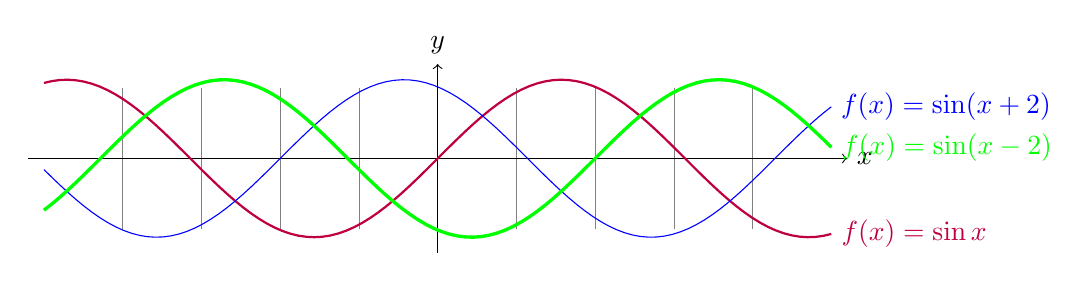
\begin{tikzpicture}[domain=-5:5,samples=100] 
    \draw[very thin,color=gray] (-4.9,-0.9) grid (4.9,0.9);
    \draw[->] (-5.2,0) -- (5.2,0) node[right] {$x$}; 
    \draw[->] (0,-1.2) -- (0,1.2) node[above] {$y$};
    \draw[thick, color=purple]   plot (\x,{sin(\x r)})    node[right] {$f(x) = \sin x$}; 
    \draw[color=blue]   plot (\x,{sin(deg(\x+2))})    node[right] {$f(x) = \sin (x+2)$}; 
    \draw[very thick, color=green]   plot (\x,{sin(deg(\x-2))})    node[right] {$f(x) = \sin (x-2)$}; 
  \end{tikzpicture}

\newcounter{k}
\setcounter{k}{-15}

\begin{animateinline}[controls,autoplay,palindrome]{10}%
  \whiledo{\thek<17}{%
  \begin{tikzpicture}[domain=-5:5,samples=100]%
    \draw[very thin,color=gray] (-4.9,-0.9) grid (4.9,0.9);%
    \draw[->] (-5.2,0) -- (5.2,0) node[right] {$x$};%
    \draw[->] (0,-1.5) -- (0,1.5) node[above] {$y$};%
    \pgfmathsetmacro\result{\thek/10};%
    \ifthenelse{\thek<0}{%
    \draw[thick, color=purple]   plot (\x,{sin(deg(\x+\thek/10)})    node[right, minimum height=0.7cm, minimum width=4cm] {$f(x) = \sin (x\pgfmathprintnumber{\result})$};}%
   {\draw[thick, color=purple]   plot (\x,{sin(deg(\x+\thek/10)})    node[right, minimum height=0.7cm, minimum width=4cm] {$f(x) = \sin (x+\pgfmathprintnumber{\result})$};}%
  \end{tikzpicture}%
  \stepcounter{k}%
  \ifthenelse{\thek<17}{\newframe}{\end{animateinline}}}%

\textbf{\textit{Paslinkimas $c$ vienetų viršun}} \back{t2b}{t2}

  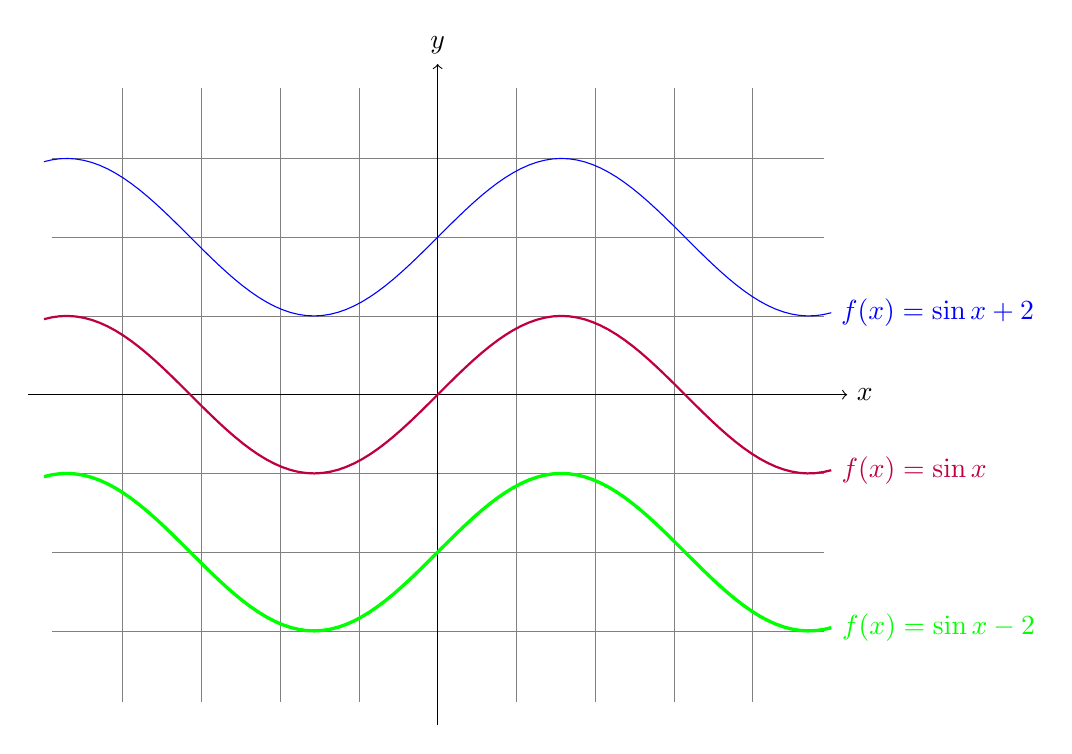
\begin{tikzpicture}[domain=-5:5,samples=100] 
    \draw[very thin,color=gray] (-4.9,-3.9) grid (4.9,3.9);
    \draw[->] (-5.2,0) -- (5.2,0) node[right] {$x$}; 
    \draw[->] (0,-4.2) -- (0,4.2) node[above] {$y$};
    \draw[thick, color=purple]   plot (\x,{sin(\x r)})    node[right] {$f(x) = \sin x$}; 
    \draw[color=blue]   plot (\x,{sin(deg(\x))+2})    node[right] {$f(x) = \sin x +2$}; 
    \draw[very thick, color=green]   plot (\x,{sin(deg(\x))-2})    node[right] {$f(x) = \sin x-2$}; 
  \end{tikzpicture}
  
\setcounter{k}{-15}

\begin{animateinline}[controls,autoplay,palindrome]{10}
  \whiledo{\thek<17}{%
  \begin{tikzpicture}[domain=-5:5,samples=100]%
    \draw[very thin,color=gray] (-4.9,-2.9) grid (4.9,2.9);%
    \draw[->] (-5.2,0) -- (5.2,0) node[right] {$x$};%
    \draw[->] (0,-2.9) -- (0,2.9) node[above] {$y$};%
    \pgfmathsetmacro\result{\thek/10};%
    \ifthenelse{\thek<0}{%
    \draw[thick, color=purple]   plot (\x,{sin(deg(\x))+\thek/10})    node[right, minimum height=0.7cm, minimum width=4cm] {$f(x) = \sin (x)\pgfmathprintnumber{\result}$};}%
   {\draw[thick, color=purple]   plot (\x,{sin(deg(\x))+\thek/10})    node[right, minimum height=0.7cm, minimum width=4cm] {$f(x) = \sin (x)+\pgfmathprintnumber{\result}$};}%
  \end{tikzpicture}%
  \stepcounter{k}%
  \ifthenelse{\thek<17}{\newframe}{\end{animateinline}}}%

\textbf{\textit{Spaudimas $k$ kartų prie $y$ ašies}}\back{t3b}{t3}

  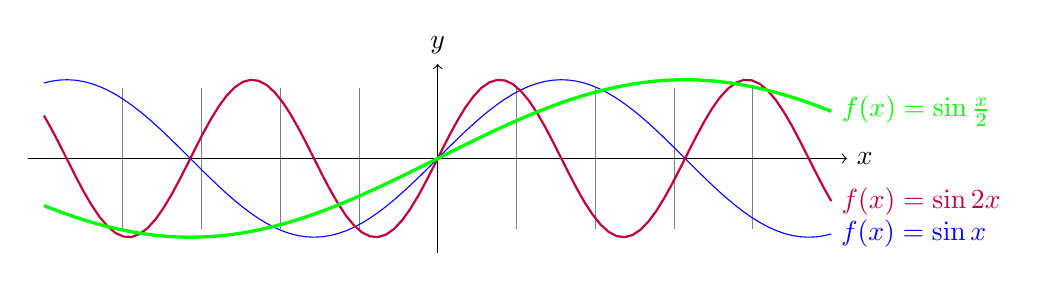
\begin{tikzpicture}[domain=-5:5,samples=100] 
    \draw[very thin,color=gray] (-4.9,-0.9) grid (4.9,0.9);
    \draw[->] (-5.2,0) -- (5.2,0) node[right] {$x$}; 
    \draw[->] (0,-1.2) -- (0,1.2) node[above] {$y$};
    \draw[color=blue]   plot (\x,{sin(\x r)})    node[right] {$f(x) = \sin x$}; 
    \draw[thick, color=purple]   plot (\x,{sin(2*\x r)})    node[right] {$f(x) = \sin 2x$}; 
    \draw[very thick, color=green]   plot (\x,{sin(\x/2 r)})    node[right] {$f(x) = \sin \frac{x}{2}$}; 
  \end{tikzpicture}
\setcounter{k}{-40}

\begin{animateinline}[controls,autoplay,palindrome]{20}%
  \whiledo{\thek<40}{%
  \begin{tikzpicture}[domain=-30:30,samples=200] %
    %\useasboundingbox (-0.5\textwidth,-2) rectangle (\textwidth,3.28);
    \pgfmathsetmacro\result{\thek/10};%
    \begin{scope}[scale=0.15, local bounding box=scope1]
    \draw[very thin,color=gray,ystep=10] (-29.9,-4.9) grid (29.9,4.9);%
    \draw[->] (-29.2,0) -- (29.2,0) node[right] {$x$};%
    \draw[->] (0,-4.9) -- (0,4.9) node[above] {$y$};%
    \draw[thick, color=purple]   plot (\x,{5*sin(deg(\x*\thek/10))});
    \end{scope}
    \node[right = 0cm of scope1, color=purple, minimum height=0.7cm, minimum width=3.5cm] {$f(x) = \sin (\pgfmathprintnumber{\result} x)$};%
  \end{tikzpicture}%
  \stepcounter{k}%
  \ifthenelse{\thek<40}{\newframe}{\end{animateinline}}}%


\textbf{\textit{Tempimas $k$ kartų nuo $x$ ašies}} \back{t4b}{t4}

  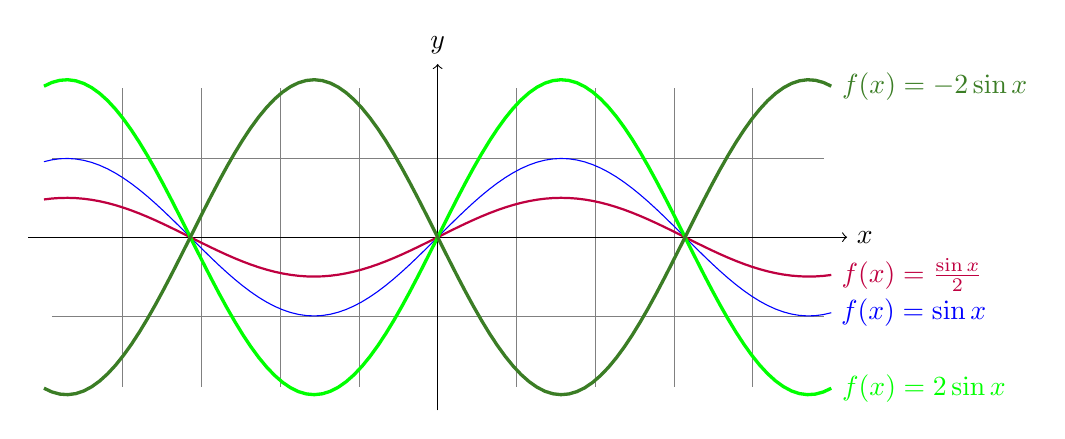
\begin{tikzpicture}[domain=-5:5,samples=100] 
    \draw[very thin,color=gray] (-4.9,-1.9) grid (4.9,1.9);
    \draw[->] (-5.2,0) -- (5.2,0) node[right] {$x$}; 
    \draw[->] (0,-2.2) -- (0,2.2) node[above] {$y$};
    \draw[color=blue]   plot (\x,{sin(\x r)})    node[right] {$f(x) = \sin x$}; 
    \draw[thick, color=purple]   plot (\x,{sin(\x r)/2})    node[right] {$f(x) = \frac{\sin x}{2}$}; 
    \draw[very thick, color=green]   plot (\x,{sin(\x r)*2})    node[right] {$f(x) = 2\sin x$}; 
    \draw[very thick, color=OliveGreen]   plot (\x,{sin(\x r)*(-2)})    node[right] {$f(x) = -2\sin x$}; 
  \end{tikzpicture}

\setcounter{k}{-15}
\begin{animateinline}[controls,autoplay,palindrome]{10}%
  \whiledo{\thek<17}{
  \begin{tikzpicture}[domain=-5:5,samples=100] 
    \draw[very thin,color=gray] (-4.9,-1.9) grid (4.9,1.9);%
    \draw[->] (-4.2,0) -- (5.2,0) node[right] {$x$};% 
    \draw[->] (0,-2.2) -- (0,2.2) node[above] {$y$};%
    \pgfmathsetmacro\result{\thek/10};%
    \draw[thick, color=purple]   plot (\x,{\thek/10*sin(deg(\x))})    node[right, color=purple, minimum height=0.7cm, minimum width=3.5cm] {$f(x) = \pgfmathprintnumber\result\cdot\sin x$};%
  \end{tikzpicture}%
  \stepcounter{k}%
  \ifthenelse{\thek<17}{\newframe}{\end{animateinline}}}
 
\textbf{\textit{Pirma pastaba}: rodyklė} visais atvejais nusako funkcijos argumentų arba reikšmių pakeitimą. 
\textbf{\textit{Antra pastaba:}} šių iliustracijų pavadinimuose pateikiamos formuluotės yra pritaikytos tik atvejams $c>0$ ir $k>1$. Norėdami nustatyti, kaip grafikų pokyčiai atrodys likusiais atvejais, transformavimą apibūdinančius žodžius pakeiskite jiems antonimiškais.

\subsection*{Papildomas skyrius: kaip paaiškinti ir įsiminti funkcijų grafikų transformacijas?}
Norint giliau suprasti priežastis, kodėl išvardyti funkcijos argumentų ar reikšmių pakeitimai atitinka funkcijos grafikų pokyčius taip, kaip nurodyta, reikėtų pradėti nuo gilesnio supratimo, kaip iš funkcijų yra gaunami jų grafikai.

Nagrinėjant visus lig tol kompiuterine programa braižytų funkcijų grafikus, svarbu pastebėti šias savybes:
\begin{itemize}
\item Funkcijos argumentai visur buvo parenkami taip, kad pokytis tarp gretimų argumentų reikšmių būtų vienodas.
\item Funkcijos argumentai kartu su funkcijos įgyjamomis reikšmėmis lentelėje buvo išsidėstę taip, kad lentelės langeliai būtų virš juos atitinkančių grafiko taškų.
\item Jei atliktume kokią nors funkcijos grafiko tranformaciją, tai lentelėje skaičiai pasikeitų ne bet kaip, o taip, kad šios dvi savybės išliktų.
\end{itemize}

Pirmosiomis dviem savybėmis įsitikinti galite pažvelgę į funkcijos $f(x)=\sin(x)$ lentelę bei grafiką:

\includegraphics[width=\textwidth]{graphtrans_1.png}

Įsitikinsime, kad atlikus transformaciją $x \to kx$, kur $k=2$, grafikas susispaus du kartus link $y$ ašies. Po transformacijos $f(x)=\sin(x)$ pasikeis į $f(x)=\sin(2x)$, o lentelė pasikeis į:

\includegraphics[width=\textwidth]{graphtrans_2.png}

Remiantis aprašytomis savybėmis pažymėtą pakeistą lentelės eilutę, nurodančią argumento reikšmes, galime ne tik \textbf{\textit{sutapatinti}} su eilute, kurioje reikšmės sutampa su pradinės (nepakeistos) eilutės reikšmėmis, bet ir pasinaudodami ankstesniais duomenimis pavaizduoti naują grafiką:

\includegraphics[width=\textwidth]{graphtrans_3.png}

Aprašytąją transformaciją $x \to kx$ laikau pačia sudėtingiausia iš 4 pagrindinių. Ji nėra įtraukta į mokyklinį kursą, tačiau supratus aprašytą įrodymo eigą, suprasti, kodėl $x \to x+c$ atitinka postūmį į kairę, daug lengviau ir tą galima padaryti samprotaujant analogiškai.

Minėtos dvi transformacijos yra vienintelės, kuriose lentelėje reikia pakeisti ne funkcijos reikšmes, o argumentus, t.y. pirmą lentelės eilutę, kontroliuojančią $x$ ašį. Jas laikau sudėtingiausiomis.

Atliekant likusias transformacijas $\Big(f(x) \rightarrow f(x)+c, x \rightarrow kx, f(x) \rightarrow |f(x)|\Big)$ keičiasi tik funkcijos reikšmės (antra lentelės eilutė), bet ne argumentai (pirma eilutė). Todėl $x$ ašis irgi nepakinta, o kinta tik taškų išsidėstymas vertikalia kryptimi. Tuo siūlau įsitikinti jums patiems.

Neišnagrinėjome tik simetrijos $y=x$ ašies atžvilgiu. Ši transformacija nėra sudėtinga, tačiau greičiausiai irgi neįeina į mokyklinį kursą.

\subsection*{Kas yra funkcijos tyrimas ir iš ko jis susideda?}
\begin{mybox}{Funkcijos tyrimas}
Funkcijos tyrimas - tai procesas, kuomet taikomi tam tikri metodai, skirti nustatyti funkcijos grafiko eskizui. Valstybiniam egzaminui būtina mokėti šiuos metodus:
\begin{itemize}
\item Nustatyti didžiausią arba mažiausią reikšmę duotame intervale.
Paprastais atvejais tai nustatyti 
\item Nustatyti funkijos didėjimo ir mažėjimo intervalus.
\item Nustatyti taškus, kuriuose funkcijos grafikas kerta $Ox$ ašį.
\item Nustatyti taškus, kuriuose funkcijos grafikas kerta $Oy$ ašį.
\item Nustatyti, kokią reikšmę įgyja funkcija duotame taške (su duota argumento reikšme).
\item Nustatyti taškus, kuriuose funkcija įgyja duotą reikšmę.
\item Ištirti funkcijos lyginumą (lyginė, nelyginė arba nei tokia, nei tokia).
\item Ištirti funkcijos periodiškumą (jei periodinė - nustatyti periodą).
\end{itemize}
\end{mybox}
Kiekvieną iš šių metodų aptarsime atskirai. 

\textbf{\textit{Pastaba:}} su funkcijos $f(x)$ išvestine $f'(x)$ dar nesusipažinome, tačiau pratimų, kuriuose reikės mokėti ją skaičiuoti, kol kas neįtrauksime. Kol kas galima žinoti tik tiek:
Jei $f'(a)>0$, tai funkcija didėja taške $a$, o jei $f'(a)<0$, tai funkcija mažėja taške $a$. Lygybės atveju taškas $a$ vadinamas funkcijos \textbf{\textit{kritiniu tašku}} ir jame funkcija nei didėja, nei mažėja.
\subsubsection*{\fbox{Didžiausia ir mažiausia reikšmė}}
\begin{minipage}[b]{0.65\linewidth}
Remiantis grafiku mažiausią ir didžiausią reikšmę rasti nesudėtinga:
\newline
\newline
\textbf{\textit{VBE 2017, 1 užd.}} Paveiksle pavaizduotas funkcijos $y=f(x)$ grafikas, kai $x \in [-2;8]$. Kokia mažiausia funkcijos reikšmė šiame intervale?
\newline
\newline
Bendru atveju (kai nesiremiama grafiku), jei duotas intervalas $[a;b]$ tai funkcijos $f(x)$ mažiausios arba didžiausios reikšmės randamos taip:
\end{minipage}
\begin{minipage}[m]{0.3\linewidth}
\includegraphics[width=\textwidth]{VBE2017_1.png}
\end{minipage}
\begin{itemize}
\item Funkcijai $f(x)$ nustatomos visos argumento reikšmės $t$, kurioms galioja $f'(t)=0$, t.y. visi kritiniai taškai.
\item Imant visus kritinius taškus bei intervalo galus $a$ ir $b$ sudaromas rinkinys taškų (argumento reikšmių), kuriuose funkcija gali įgyti didžiausią arba mažiausią reikšmę.
\item Kiekvienai argumento reikšmei nustatoma jį atitinkanti funkcijos reikšmė ir iš gautų reikšmių išrenkama pati didžiausia arba pati mažiausia. 
\item Kartais uždavinio sąlygoje prašo ne nustatyti didžiausią arba mažiausią reikšmę, o tašką, kuriame ji įgyjama. Tuomet rastai funkcijos reikšmei reikia pateikti ją atitinkančią funkcijos argumento reikšmę.
\end{itemize}
\subsubsection*{\fbox{Didėjimo ir mažėjimo intervalai}}
\begin{itemize}
\item Funkcijos \textbf{\textit{didėjimo}} intervalai yra tai, ką gauname išsprendę nelygybę $f'(a)>0$
\item Funkcijos \textbf{\textit{mažėjimo}} intervalai yra tai, ką gauname išsprendę nelygybę $f'(a)<0$
\end{itemize}
\subsubsection*{\fbox{$Ox$ ašies kirtimo taškai}}
Argumento reikšmės, su kuriomis funkcijos reikšmė lygi nuliui, dar vadinamos funkcijos nuliais. Šios reikšmės yra lygties $f(x)=0$ sprendiniai. Kiekvieną sprendinį $x=a$ atitinka taškas $(a; 0)$
\subsubsection*{\fbox{$Oy$ ašies kirtimo taškai}}
Funkcijai $f(x)$ imdami argumento reikšmę $x=0$ gausime jos reikšmę $f(0)$. Vadinasi, kai funkcijos grafikui priklauso taškas $(0;f(0))$. Šis taškas yra $Oy$ ašyje, be to, jis yra vienintelis, priklausantis šiai ašiai.
\subsubsection*{\fbox{Funkcijos įgyjama reikšmė duotame taške}}
Egzamine dažnai klausia, kokią reikšmę įgyja funkcija $f(x)$ taške $x=a$. Atsakymas į šį klausimą būtų: tai, ką gauname apskaičiavę $f(a)$. Tačiau pasitaiko ir šiek tiek sudėtingesnių atvejų.

\textbf{\textit{VBE 2016 16 užd. dalis}} Duotos funkcijos $f(x)=x^2$ ir $g(x)=x+1$. Nustatyti funkcijas $f(g(x))$ ir $g(f(x))$. 

\textbf{\textit{Sprendimas.}} Pirmu atveju išraiškoje $f(x)=x^2$ įstatome argumento $x$ reikšmę $g(x)$. Turime $f(g(x))=g(x)^2$. Dešinėje pusėje galime pakeisti $g(x)$ į $x+1$, todėl gausime $f(g(x))=(x+1)^2$. Analogiškai samprotaudami galime gauti, kad $g(f(x))=x^2+1$.
\subsubsection*{\fbox{Taškai, kuriuose funkcija įgyja duotą reikšmę}}
Jei klausia, su kuriomis argumento $x$ reikšmėmis funkcija $f(x)$ įgyja reikšmę $a$, tai spręsime lygtį $f(x)=a$. Jos sprendiniai ir bus ieškomos reikšmės.

\textbf{\textit{VBE 2016 16.2 užd.}} Duotos funkcijos $f(x)=x^2$ ir $g(x)=x+1$. Išspręskite lygtį $g(f(x))=2$. 

\textbf{\textit{Sprendimas.}} Pagal ankstesnes išvadas $g(f(x))=x^2+1$. Todėl sprendžiame lygtį $x^2+1=2$. Šios lygties prasmė: ieškomos argumento $x$ reikšmės, su kuriomis funkcija $y=x^2+1$ įgyja reikšmę 2. Išsprendę lygtį gauname net dvi tokias reikšmes: $-1$ ir $1$.
\subsubsection*{\fbox{Funkcijos lyginumas}}
Susipažinus su funkcijų transformacijomis turėtų tapti aišku, jog funkcijos $f(x)$ grafikas yra 
\begin{itemize}
\item simetriškas funkcijos $f(-x)$ grafikui $Oy$ ašies atžvilgiu
\item simetriškas funkcijos $-f(-x)$ grafikui taško $(0;0)$ atžvilgiu
\item simetriškas funkcijos $-f(x)$ grafikui $Ox$ ašies atžvilgiu
\end{itemize}
Kai $f(x)=f(-x)$ funkcija vadinama lygine, o kai $f(x)=-f(-x)$ - nelygine. Likusiais atvejais - nei lygine, nei nelygine.
\subsubsection*{\fbox{Funkcijos periodiškumas}}
Susipažinus su funkcijų transformacijomis turėtų tapti aišku, jog, kai $f(x)=f(x+T)$, tai funkcijos $f(x)$ grafikas sutampa su jo poslinkiu per $T$ į kairę. Mažiausias toks $T>0$, su kuriuo $f(x)=f(x+T)$, yra vadinamas funkcijos \textbf{\textit{periodu}}. Žiūrėdami į pateiktus pagrindinių funkcijų eskizus turėtumėte įsitikinti, kad tik trigonometrinės funkcijos $f(x)=\sin (x)$, $f(x)=\cos (x)$ ir $f(x)=\text{tg} (x)$ turės periodus. Kam jie lygūs?
\end{document}